\documentclass[../main.tex]{subfiles}
\graphicspath{{\subfix{../diagrams/}}}


\begin{document}

\chapter{Introduction}
Hello, here is some text without a meaning...\cite{salemi2013uvm}

\textbf{Hello world!}

\begin{figure}[bh]
\centering
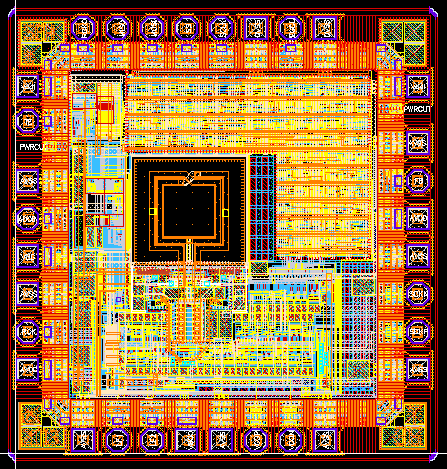
\includegraphics[width=5cm]{diagrams/MPW2Naretlayout.png}

\label{fig:img1}
\caption{some figure}
\end{figure}

\section{Background}
\blindtext[6]

\section{Motivation}
\blindtext[3]

\section{Goals And Contribution}
\blindtext[3]

\section{Motivation}
\blindtext[3]

\section{Structure}
We tried to structure this book to match the integrated circuits (ICs) design flow. 
\\
\\
Chapter1 gives essential information about cryptography starting with Section 1.1 that talks about the state of art in cryptography methods and Section 1.2 mentions the details of the used cryptography algorithm in our System on Chip (SoC). 
\\
\\
Chapter 2 mentions the tools we used in the whole flow going from design to verification to tape out, it also gives a brief introduction about the open source community and their emerging EDAs.
\\
\\
Chapter 3 starts with 3.1 giving a quick introduction to RISC-V architecture and open source hardware design. Section 3.2 describes the overall architecture of our SoC and mentions important IPs. Section 3.3  gives in-depth details about AlexCore, Section 3.3.1 gives details about the integer pipelines and basic control operations, Section 3..3.2  gives details about privilege instructions and implemented CSRs for Linux support, Section 3.3.3 describes how we manage interrupts in AlexCore. Section 3.3 gives important background information about OpenPiton framework benefits and core integrations, Section 3.4 talks about the architecture and design of the used cryptography IP, Section 3.5 gives details and results of testing AlexCore compliance with RISC-V ISA.
\\
\\
Chapter 4 offers more details on the design phase, taking the design to and FPGA synthesis and  build.
\\
\\
Chapter 5 discusses more verification techniques using the universal verification method 
\\
\\
Chapter 6 discusses the back-end implementation of the SoC on UMC180 PDK.
\\
\\
Chapter 6 presents the conclusion of the book and discusses possible future improvements


\end{document}
